\documentclass{article}
\author{Alejandro Zubiri}
\date{Tue Oct 08 2024}
\title{Movimiento Circular}

\usepackage{amsmath}
\usepackage{tikz}
\usepackage{physics}

\begin{document}
\maketitle
\tableofcontents
\pagebreak
\section{Resumen}
\begin{flalign}
    \nonumber&\vec{v}=\vec{\omega}\times \vec{r}&&\\
    \nonumber&T= \frac{2\pi}{\omega}= \frac{1}{f}&&\\
    \nonumber&\dv{\theta}{t}=\frac{1}{R}\dv{s}{t}&&\\
    \nonumber&\vec{v}=|v|\vec{u_t}&&\\
    \nonumber&\dv{\vec{u_t}}=\dv{\theta}{t}\vec{u_n}=\frac{1}{R}\dv{s}{t}\vec{u_n}&&\\
    \nonumber&\vec{a}=\vec{\alpha}\times \vec{R}+ \vec{\omega}\times (\vec{\omega}\times \vec{R})&&\\
    \nonumber&=\vec{a}=\vec{\alpha}\times \vec{R}+ \vec{\omega}\times (\vec{\omega}\times \vec{R})&&
\end{flalign}

\tikzset{every picture/.style={line width=0.75pt}} %set default line width to 0.75pt        

\begin{center}
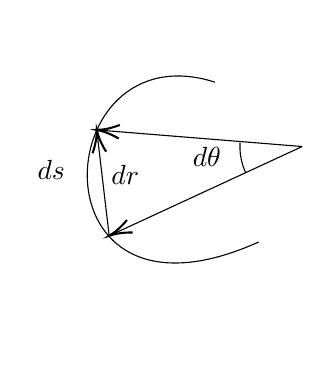
\begin{tikzpicture}[x=0.75pt,y=0.75pt,yscale=-1,xscale=1]
%uncomment if require: \path (0,300); %set diagram left start at 0, and has height of 300

%Curve Lines [id:da3464038578004158] 
\draw    (308,181.6) .. controls (197,231.6) and (206,78.6) .. (287,104.6) ;
%Straight Lines [id:da013023585384112968] 
\draw    (329,135.6) -- (237.82,177.76) ;
\draw [shift={(236,178.6)}, rotate = 335.19] [color={rgb, 255:red, 0; green, 0; blue, 0 }  ][line width=0.75]    (10.93,-3.29) .. controls (6.95,-1.4) and (3.31,-0.3) .. (0,0) .. controls (3.31,0.3) and (6.95,1.4) .. (10.93,3.29)   ;
%Straight Lines [id:da5935975860519136] 
\draw    (329,135.6) -- (231.99,127.76) ;
\draw [shift={(230,127.6)}, rotate = 4.62] [color={rgb, 255:red, 0; green, 0; blue, 0 }  ][line width=0.75]    (10.93,-3.29) .. controls (6.95,-1.4) and (3.31,-0.3) .. (0,0) .. controls (3.31,0.3) and (6.95,1.4) .. (10.93,3.29)   ;
%Shape: Arc [id:dp8509896178013645] 
\draw  [draw opacity=0] (301.73,148.13) .. controls (299.98,144.32) and (299,140.07) .. (299,135.6) .. controls (299,134.95) and (299.02,134.31) .. (299.06,133.68) -- (329,135.6) -- cycle ; \draw   (301.73,148.13) .. controls (299.98,144.32) and (299,140.07) .. (299,135.6) .. controls (299,134.95) and (299.02,134.31) .. (299.06,133.68) ;  
%Straight Lines [id:da577271865101106] 
\draw    (236,178.6) -- (230.23,129.59) ;
\draw [shift={(230,127.6)}, rotate = 83.29] [color={rgb, 255:red, 0; green, 0; blue, 0 }  ][line width=0.75]    (10.93,-3.29) .. controls (6.95,-1.4) and (3.31,-0.3) .. (0,0) .. controls (3.31,0.3) and (6.95,1.4) .. (10.93,3.29)   ;

% Text Node
\draw (275.04,134.72) node [anchor=north west][inner sep=0.75pt]    {$d\theta $};
% Text Node
\draw (235.84,143.32) node [anchor=north west][inner sep=0.75pt]    {$dr$};
% Text Node
\draw (200.24,141.12) node [anchor=north west][inner sep=0.75pt]    {$ds$};


\end{tikzpicture}
\end{center}
Para empezar con algunas definiciones básicas, definimos la velocidad lineal de una partícula en un movimiento circular de la siguiente forma:
\begin{equation}
    \begin{split}
        \vec{v}=\vec{\omega}\times \vec{r}
    \end{split}
\end{equation}
Donde $\vec{\omega}$ es el vector velocidad angular y $\vec{r}$ es el vector posición. Ambas son funciones de tiempo. Más precisamente:
\begin{equation}
    \begin{split}
        \vec{\omega}=\frac{d\vec{\theta}}{dt}=\frac{d\theta}{dt}\vec{k}
    \end{split}
\end{equation}

\section{Movimiento Circular Uniforme}
Este movimiento se caracteriza por $\ddot{\theta}=0\Rightarrow\dot{\theta}=\omega=cte$.\\
\begin{equation}
    \begin{split}
        \ddot{\theta}=\dv{\theta}{t}=\omega
    \end{split}
\end{equation}
Si despejamos para $\omega$ e integramos, obtenemos el cambio en el ángulo en función del tiempo:
\begin{equation}
    \begin{split}
        \int_{0}^{\theta}\dd{\theta}=\int_{0}^{t}\omega\dd{t}
    \end{split}
\end{equation}
Si establecemos $\theta=2\pi$, es decir, una vuelta entera
\begin{equation}
    \begin{split}
        2\pi=\omega t
    \end{split}
\end{equation}
Y si despejamos en función de $t$
\begin{equation}
    \begin{split}
        t=\frac{2\pi}{\omega}=T
    \end{split}
\end{equation}
Obtenemos el tiempo que tarda nuestra partícula en dar una vuelta, que es lo que entendemos por \textbf{período}.\\
Además, tenemos la siguiente relación:
\begin{equation}
    \begin{split}
        ds=Rd\theta
    \end{split}
\end{equation}
Que podemos despejar como
\begin{equation}
    \begin{split}
        d\theta=\frac{ds}{R}
    \end{split}
\end{equation}
Si dividimos ambos lados por $dt$:
\begin{equation}
    \begin{split}
        \frac{d\theta}{dt}=\frac{1}{R} \frac{ds}{dt}
    \end{split}
\end{equation}
Obteniendo así:
\begin{equation}
    \begin{split}
        R \frac{d\theta}{dt}= \frac{ds}{dt}
    \end{split}
\end{equation}
Por definición, la velocidad es
\begin{equation}
    \begin{split}
        \vec{v}=\vec{u_{t}}|v|
    \end{split}
\end{equation}
Donde $u_{t}$ representa el vector director unitario de la velocidad. Despejando con respecto a este, tenemos que
\begin{equation}
    \begin{split}
        \vec{u_{t}}= \frac{\vec{v}}{|v|}=\frac{1}{|v|}(v_x,v_y)=(\cos \theta, \sin \theta)
    \end{split}
\end{equation}
El vector normal a este
\begin{equation}
    \begin{split}
        \vec{u_n}=(-\sin \theta, \cos \theta)
    \end{split}
\end{equation}
La derivada con respecto al tiempo del vector unitario es:
\begin{equation}
    \begin{split}
        \frac{d u_t}{dt}=( \frac{d\cos \theta}{dt} \frac{d \theta}{dt},\frac{d\sin \theta}{dt} \frac{d \theta}{dt})=
        \frac{d \theta}{dt}(-\sin \theta, cos \theta)= \frac{d \theta}{dt} \vec{u_n}
    \end{split}
\end{equation}
Obteniendo la siguiente relación:
\begin{equation}
    \begin{split}
        \frac{d u_t}{dt}=\frac{d \theta}{dt} \vec{u_n}=\frac{1}{r}\dv{s}{t}\vec{u_n}
    \end{split}
\end{equation}
Vamos a desarrollar la \textbf{aceleración}.
La aceleración es, por tanto:
\begin{equation}
    \begin{split}
        \vec{a}= \frac{d \vec{v}}{dt}=\frac{d}{dt}(\vec{u_{t}}|v|)= \frac{d u_{t}}{dt}|v|+ u_{t} \frac{d|v|}{dt}
    \end{split}
\end{equation}
Si utilizamos los resultados de la ecuación 11, obtenemos que
\begin{equation}
    \begin{split}
        \vec{a}= \dv{|v|}{t}\vec{u_t} + \frac{|v|^{2}}{R}\vec{u_n}
    \end{split}
\end{equation}
Donde identificamos $\dv{|v|}{t}\vec{u_t}$ como la aceleratión tangencial $\vec{a_t}$ y $\frac{|v|^{2}}{R}\vec{u_n}$ como
la aceleración normal $\vec{a_n}$
\section{Movimiento Circular Uniformemente Acelerado}
En este caso, la aceleración no es cero, y por tanto nuestra velocidad angular \textbf{no} es constante. Definimos la
aceleración angular $\vec{\alpha}$ como:
\begin{equation}
    \begin{split}
        \vec{\alpha}=|\alpha|\vec{k}=\dv[2]{\theta}{t}\vec{k}
    \end{split}
\end{equation}
La aceleración tangencial es
\begin{equation}
    \begin{split}
        \vec{a}=\dv{\vec{v}}{t}=\dv{t} (\vec{\omega}\times \vec{R})= \dv{\omega}{t}\times \vec{R}+ \omega\times\dv{R}{t}
    \end{split}
\end{equation}
Si recordamos, $\dv{\vec{\omega}}{t}=\vec{\alpha}$ y $\dv{\vec{R}}{t}=\vec{v}=\vec{\omega}\times \vec{R}$. Si realizamos
estas substituciones, obtenemos
\begin{equation}
    \begin{split}
        \vec{a}=\vec{\alpha}\times \vec{R}+ \vec{\omega}\times (\vec{\omega}\times \vec{R})
    \end{split}
\end{equation} 
Lo que nos daría como resultado una ecuación de movimiento $\theta(t)$
\begin{equation}
    \begin{split}
        \theta(t)=\theta_0+\omega_0t+ \frac{1}{2}\alpha t ^{2}
    \end{split}
\end{equation} 
\end{document}
